% DSD Lab3 report

\documentclass[10pt]{article}
\usepackage{mathtools, amsmath, amsfonts, amssymb}
\usepackage{hyperref, graphicx, wrapfig, geometry}
\usepackage[makeroom]{cancel}

\usepackage[section]{placeins}
\newgeometry{margin=2cm}

\title{ECSE 323 --- Group 47 Lab 3 Report}
\author{Junyoung Shin id. 260499663\\ Timothee Flichy id. 260557686}
\date{\today}

\begin{document}
\maketitle
\section*{Design and simulation of a 0-to-25 Counter Circuit}
We desiged a 0-to-25 counter with inputs clock, asynchronous reset, and count_enable. The counter gives an output of a 5bit which counts up avery clock cycle while count_enable is high and reset is high. The count will add 1bit every clock cycle until it reaches the max value of $"11001"$. The count_enable and count are trigered at the rising edge of the clock. When reset goes low, the count goes to $"00000"$. If count_enable is not set high, the count is will at the value it was not until count_enable goes high.
To test our code, we created a clock pulse of 50ns and tested the VHDL code. The data of the test cana be seen on figure \ref{fig:count_test}.
\begin{figure}[!htb]
    \centering
    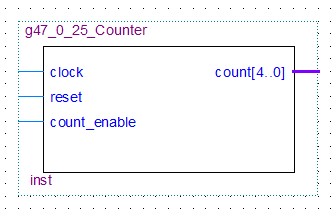
\includegraphics[width=0.6\textwidth]{./counter_0to25.png}
    \caption{0-to-25 counter driver pins.}
    \label{fig:count_pin}
\end{figure}
\begin{figure}[!htb]
    \centering
    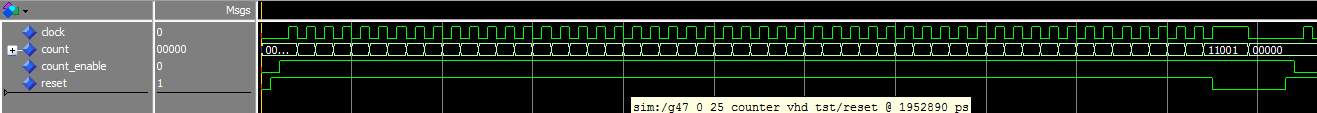
\includegraphics[width=0.6\textwidth]{./test_0to25.png}
    \caption{Simulation of the 0-to-25 counter.}
    \label{fig:count_test}
\end{figure}
\secntion*{Testing the 7-segment LED decoder on the Altera Board}
The Altera DE1 development board is equiped with 4 7-segment LED display and 10 simple switches are controlled and received by the FPG. Our goal was to make a test bed to make the LED to display letters in the alphabet when playing with 5 of the switches availabe on the board. The lettering configuration was as followed on table \ref{fig:alph_label}.
\begin{table}[!htb]
    \caption{Color label corresponding to code inputs}
    \label{tab:alph_label}
    \centering
    \begin{tabular}{l|cc}
    \hline
    \hline
    \textbf{Code} & \textbf{Letter}\\
    \hline
        \verb@00000@ & A \\
        \verb@00001@ & B \\
        \verb@00010@ & C \\
        \verb@00011@ & D \\
        \verb@00100@ & E \\
        \verb@00101@ & F \\
        \verb@00110@ & G \\
        \verb@00111@ & H\\
        \verb@01000@ & I\\
        \verb@01001@ & J\\
        \verb@01010@ & K\\
        \verb@01011@ & L\\
        \verb@01100@ & M\\
        \verb@01101@ & N\\
        \verb@01110@ & O\\
        \verb@01111@ & P\\
        \verb@10000@ & Q\\
        \verb@10001@ & R\\
        \verb@10010@ & S\\
        \verb@10011@ & T\\
        \verb@10100@ & U\\
        \verb@10101@ & V\\
        \verb@10110@ & W\\
        \verb@10111@ & X\\
        \verb@11000@ & Y\\
        \verb@11001@ & Z\\
    \hline
    \hline
    \end{tabular}
\end{table}
To decode the binary numbers being put in by the swtiches, we used the 26_5 decoder from the 



\end{document}